% =====================================================================
%  Graphical abstract v2 -- "Strain-coupled one-dimensional turbulence
%  for rapid distortion"
%
%  Standalone: compile with  pdflatex graphical_abstract.tex
%
%  Story: ONE ODT line convecting downstream, shown as five snapshots
%  t = 0 ... t_n inside the contracting strain envelope. The domain
%  shrinks as L(t) = L0 exp(int A22 dt), the scales refine, the upwash
%  component (red) is amplified. The governing operator-split equation
%  sits on top; the single-line closure of the rapid pressure--strain
%  (the soul) is highlighted below; the regime parameter chi is badged.
%
%  All knobs collected below. Each block is its own scope: delete freely.
% =====================================================================
\documentclass[border=8pt]{standalone}
\usepackage{amsmath}
\usepackage{tikz}
\usetikzlibrary{arrows.meta,decorations.pathreplacing,calc}

% ------------------------------ KNOBS --------------------------------
\definecolor{cu}{HTML}{1F77B4}      % u-component blue
\definecolor{cv}{HTML}{D62728}      % v (upwash) red
\definecolor{cstrain}{HTML}{FF7F0E} % strain / highlight orange
\definecolor{cgrey}{HTML}{666666}

\def\xA{1.4}\def\xB{4.1}\def\xC{6.8}\def\xD{9.5}\def\xE{12.2} % snapshot x
\def\envrate{0.105}   % envelope contraction rate  h(x)=\hzero*exp(-rate*(x-\xA))
\def\hzero{2.05}      % initial half-height (L0/2)
\def\ampU{0.30}       % initial u amplitude
\def\ampV{0.30}       % initial v amplitude
\def\vgrow{1.55}      % how much the upwash amplifies by t_n
\def\ushrk{0.75}      % how much u shrinks by t_n
% ----------------------------------------------------------------------

\begin{document}
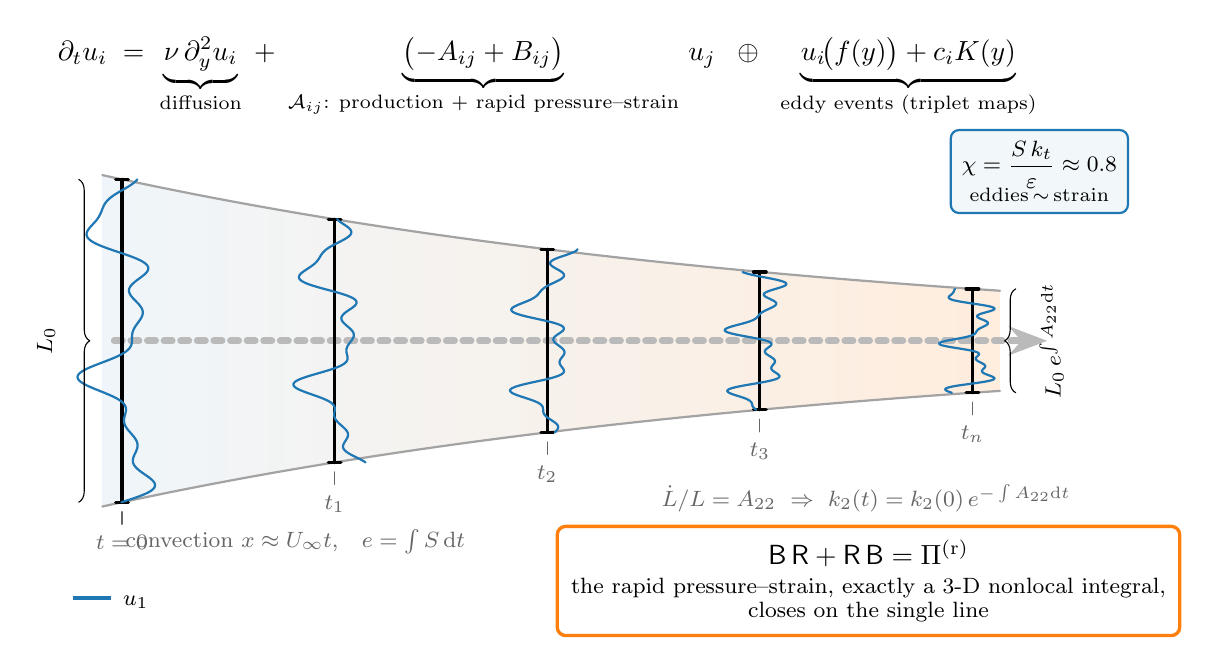
\begin{tikzpicture}[>=Stealth, line cap=round, line join=round,
                    font=\footnotesize]

% =================== contracting strain envelope ===================
\shade[left color=cu!7, right color=cstrain!14]
  plot[samples=80, domain=\xA-0.25:\xE+0.35]
    (\x,{ \hzero*exp(-\envrate*(\x-\xA)) })
  -- plot[samples=80, domain=\xE+0.35:\xA-0.25]
    (\x,{ -\hzero*exp(-\envrate*(\x-\xA)) }) -- cycle;
\draw[cgrey!60, thick]
  plot[samples=80, domain=\xA-0.25:\xE+0.35]
    (\x,{ \hzero*exp(-\envrate*(\x-\xA)) });
\draw[cgrey!60, thick]
  plot[samples=80, domain=\xA-0.25:\xE+0.35]
    (\x,{ -\hzero*exp(-\envrate*(\x-\xA)) });

% convection arrow along the centreline (behind the lines)
\draw[->, line width=2.4pt, cgrey!45, dashed]
  (\xA-0.1,0) -- (\xE+0.95,0);

% =================== five snapshots of the ODT line ===================
% x pos / phase offset (deg) -- height & scales derived from the envelope
\foreach \xc/\ph [count=\i from 0] in {\xA/0,\xB/55,\xC/130,\xD/205,\xE/290}{
  \pgfmathsetmacro\hh{\hzero*exp(-\envrate*(\xc-\xA))}       % half height
  \pgfmathsetmacro\ff{\hzero/\hh}                            % wavenumber factor
  \pgfmathsetmacro\au{\ampU*(1-(1-\ushrk)*\i/4)}             % u amp (shrinks)
  \pgfmathsetmacro\av{\ampV*(1+(\vgrow-1)*\i/4)}             % v amp (grows)
  % domain line + end caps
  \draw[very thick] (\xc,-\hh) -- (\xc,\hh);
  \draw[very thick] (\xc-0.08,-\hh) -- (\xc+0.08,-\hh);
  \draw[very thick] (\xc-0.08,\hh) -- (\xc+0.08,\hh);
  % u trace (blue) -- scales refine as the line compresses
  \draw[cu, thick, samples=200, domain=-\hh:\hh]
    plot ({\xc + \au*sin(3.1*\ff*\x r + \ph)
               + 0.55*\au*sin(6.7*\ff*\x r + 2*\ph + 80)
               + 0.35*\au*sin(11*\ff*\x r + 3*\ph + 200)}, \x);
  % v / upwash trace (red) -- amplified by the distortion
%   \draw[cv, thick, samples=200, domain=-\hh:\hh]
%     plot ({\xc + \av*sin(3.6*\ff*\x r + \ph + 120)
%               + 0.50*\av*sin(7.9*\ff*\x r + 2*\ph + 310)
%               + 0.30*\av*sin(12.5*\ff*\x r + 3*\ph + 30)}, \x);
  % time tick under the envelope
  \draw[cgrey] (\xc,{-\hzero*exp(-\envrate*(\xc-\xA))-0.12})
            -- (\xc,{-\hzero*exp(-\envrate*(\xc-\xA))-0.28});
}
% time labels
\node[cgrey, below] at (\xA,{-\hzero-0.30}) {$t=0$};
\node[cgrey, below] at (\xB,{-\hzero*exp(-\envrate*(\xB-\xA))-0.30}) {$t_1$};
\node[cgrey, below] at (\xC,{-\hzero*exp(-\envrate*(\xC-\xA))-0.30}) {$t_2$};
\node[cgrey, below] at (\xD,{-\hzero*exp(-\envrate*(\xD-\xA))-0.30}) {$t_3$};
\node[cgrey, below] at (\xE,{-\hzero*exp(-\envrate*(\xE-\xA))-0.30}) {$t_n$};

% braces: initial and final domain length
\draw[decorate,decoration={brace,mirror,amplitude=4pt}]
  (\xA-0.55,-\hzero) -- (\xA-0.55,\hzero)
  node[midway,left=5pt,rotate=90,anchor=south] {$L_0$};
\pgfmathsetmacro\hE{\hzero*exp(-\envrate*(\xE-\xA))}
\draw[decorate,decoration={brace,amplitude=4pt}]
  (\xE+0.55,-\hE) -- (\xE+0.55,\hE)
  node[midway,right=5pt,rotate=90,anchor=north]
  {$L_0\,e^{\int A_{22}\mathrm dt}$};

% =================== the governing mathematics ===================
% operator-split evolution equation, spanning the top
\node[align=center] at ({0.5*(\xA+\xE)},3.35) {\normalsize
  $\displaystyle
   \partial_t u_i \;=\;
   \underbrace{\nu\,\partial_y^2 u_i}_{\text{diffusion}}
   \;+\;
   \underbrace{\bigl(-A_{ij}+B_{ij}\bigr)}_{
     \mathcal A_{ij}:\ \text{production + rapid pressure--strain}}\,u_j
   \;\;\oplus\;\;
   \underbrace{u_i\!\bigl(f(y)\bigr)+c_iK(y)}_{
     \text{eddy events (triplet maps)}}$};

% the soul: single-line closure of the rapid pressure--strain
\node[draw=cstrain, very thick, rounded corners=3pt, fill=white,
      align=center, inner sep=5pt]
  at ({0.8*(\xA+\xE)},-3.05) {\normalsize
  $\mathsf{B}\,\mathsf{R}+\mathsf{R}\,\mathsf{B}=\Pi^{(\mathrm r)}$\\[1pt]
  \footnotesize the rapid pressure--strain, exactly a 3-D nonlocal
  integral,\\[-1pt]\footnotesize closes on the single line};

% wavenumber-compression math, under the contracting envelope (right)
\node[cgrey, align=center] at (10.85,-2.0)
  {$\dot L/L=A_{22}\ \Rightarrow\ k_2(t)=k_2(0)\,e^{-\int A_{22}\mathrm dt}$};

% convection label, under the envelope (left)
\node[cgrey, align=center] at (3.6,-2.55)
  {convection $x\approx U_\infty t$,\quad $e=\int S\,\mathrm dt$};

% regime badge: chi
\node[draw=cu, thick, rounded corners=3pt, fill=cu!6, align=center,
      inner sep=4pt] at (\xE+0.85,2.15)
  {$\chi=\dfrac{S\,k_t}{\varepsilon}\approx0.8$\\[-1pt]
   \scriptsize eddies\,$\sim$\,strain};

% component legend, bottom left (clear of the top equation's underbraces)
\node[anchor=west, align=left] at (\xA-0.75,-3.45)
  {\textcolor{cu}{\rule[2pt]{14pt}{1.6pt}}\, $u_1$\\[-1pt]};
%   \textcolor{cv}{\rule[2pt]{14pt}{1.6pt}}\, $u_2$ (upwash,\\[-2pt]
%   \hphantom{\rule{18pt}{0pt}}amplified)};

\end{tikzpicture}
\end{document}